\documentclass[13pt]{article}
\usepackage[utf8]{inputenc}


%% Language and font encodings
\usepackage[english]{babel}
\usepackage[utf8x]{inputenc}
\usepackage[T1]{fontenc}

%% Sets page size and margins
\usepackage[a4paper,top=2cm,bottom=2cm,left=1.5cm,right=1.5cm,marginparwidth=1.75cm]{geometry}

%% Useful packages
\usepackage{amsmath}
\usepackage{graphicx}
\usepackage[colorinlistoftodos]{todonotes}
\usepackage[colorlinks=true, allcolors=blue]{hyperref}
\usepackage{parskip}
\usepackage{subfig}

\title{\vspace{-2.0cm}Machine Learning Models\vspace{-2ex}}
\author{\vspace{-5.0cm}Adam Pluck and James O'Reilly\vspace{-3ex}}
\date{\vspace{-2ex}}

\begin{document}

\maketitle

\begin{enumerate}

\item {\Large Question 1}

\begin{enumerate}


  \item {\large What assumption does a Gaussian likelihood encode, i.e What motivates the choice of this likelihood function?}
  
  The given data pairs are corrupted by additive noise. We can assume this additive noise follows a Gaussian distribution due to the Central Limit Theorem which states that in some situations, when independent random variables are added, their properly normalised sum tends toward a normal distribution.
  
  \item {\large What does it mean that we have chosen a spherical co-variance matrix for the likelihood, contrast with the non-spherical case?}
  A diagonal co-variance matrix implies that each of the dimensions are independent of each other. The fact that it is spherical and of the form $\lambda(\mathbf{I})$ implies that each of the dimensions are independent and also the dimensions are equally varying.
  
  In the case that the co-variance matrix is non-spherical, then each of the dimensions do not vary equally.
 \end{enumerate}
 
  \item {\large If we do not assume that the data points are independent how would the likelihood look then?}
  
   $$\prod_{i = 1}^{N} p\left( y_i | f, x_i, \{y_1, ...., y_{i-1}\} \right) $$
     
  \begin{equation}
      P(\mathbf{E}) = P\left (  \bigcap_{i}^{n} E_{i}    \right )
  \end{equation}
  
  \item {\large What is the specific form of the likelihood above, complete the right-hand side of the expression? \par}
  Maybe change this as he has an equals sign in the question and we should be using a tilda? perhaps he wants us to write out the long winded version with the product.
  
  \begin{equation}
      p(\left(\mathbf{Y}|\mathbf{X},\mathbf{W}\right ) = N\left(\mathbf{Y}|\mathbf{WX}, \sigma ^2 I  \right )
  \end{equation}
  
  \item {\large Explain the concept of conjugate distributions in this context, why do they help us compute the posterior distribution?\par} Look at the lecture on October 9th. Mention the fact that the posterior integrates to one. Maybe this lecture also relates to question 17.
  
  would normally have this normalising factor in the the denominator (evidence)
  we can ignore that and calculate the proportionality. AS the posterior is a probability we know that it integrates to one and so the likelihood x prior must also integrate to one. Then we can calculate the normalising factor k.
  
  Usually, in order to calculate the posterior, we must also calculate the evidence.
  
  \begin{equation}
  Posterior = (Likelihood \cdot Prior)/Evidence
  \end{equation}
  
  For a given probability distribution $p(\mathbf{x}|\mathbf{y})$ if we can find a prior $p(\mathbf{y})$ that is conjugate to the likelihood function, then the posterior distribution will have the same form as the prior. And so with the conjugate prior we have that
  
  \begin{equation}
  Posterior \propto Likelihood \cdot Prior
  \end{equation}
  
  and so we no longer need to calculate the evidence in order to find the posterior. Conjugate priors are useful in this way because they reduce Bayesian updating to modifying the parameters of the prior distribution rather than computing ugly integrals.
  
  \item {\large Reason about the Gaussian distribution in this context, which distance function does it encode with a spherical co-variance matrix?}
  
  For a D-dimensional vector x, the multivariate Gaussian distribution takes the form
  \begin{equation}
  N(\mathbf{x}\mid\mathbf{\mu}, \mathbf{\Sigma}) =  \frac{1}{{{(2\pi) }^{D/2} }}\frac{1}{|\Sigma|^{\frac{1}{2}}}e^{-\frac{1}{2}(\mathbf{x} - \mathbf{\mu})^{T}\Sigma ^{-1}(\mathbf{x} - \mathbf{\mu})}
  \end{equation}
  And so we have that our prior is of the form 
  \begin{equation}
  p(\mathbf{W}) = \frac{1}{{{(2\pi) }^{D/2} }}\frac{1}{|\Sigma|^{\frac{1}{2}}}e^{-\frac{1}{2}(\mathbf{W} - \mathbf{W}_{0})^{T}\Sigma ^{-1}(\mathbf{W} - \mathbf{W}_{0})}
  \end{equation}
  
  From this we can see that the functional dependence of the Gaussian on W is entirely on the exponent. The exponent is in fact the Mahalanobis distance given by
  
  \begin{equation}
      D_m(x,\mathbf{x_0},\mathbf{\Sigma}) = \sqrt[]{(x-\mathbf{x_0})^T \mathbf{\Sigma}^{-1} (x-\mathbf{x_0})}
  \end{equation}
  
  However, in the case of spherical co-variance matrix, the Mahalanobis distance function reduces down to the Euclidean distance scaled by some constant.
  
  \item {\large Write out the posterior over the parameters W. Justify the posterior by providing an intuition of its form.}
  
  Need the derivation from Adam
  
  \item {\large SECTION 2: NON-PARAMETRIC LEARNING}
  Question 7: What is a non-parametric model and what is the difference between non-parametrics and parametrics?
  
  Non-parametric models assume that the distribution of the data cannot be defined in terms of a finite set of parameters. In doing so, non-parametric machine learning algorithms don't make strong assumptions about the form of the underlying function. This lack of constraint means that they are free to learn any functional form from the training data. 
  
  Representation/Parametrisation of data:
  With non-parametric methods we have the advantage of not having to assume the algebraic form of the function (the number of parameters isn't fixed), this allows the model to be more flexible. Furthermore, as no assumptions are made about the underlying function, the model will get more accurate as we feed it more data. In contrast, parametric machine learning algorithms first assume the underlying function has a fixed number of parameters and then learn the parameters from the training data. No matter how much data you throw at a parametric model, it won't change its mind about how many parameters it needs.  
  
  Interpretability of models:
  While parametric models are constrained to a fixed form and have limited complexity, due to their simple linear nature, they are much easier to interpret and understand. We can see how the parameters change over time and interpret what this means. As we have made assumptions about the form of the model, interpreting the model does not require much effort. With non-parametric models this is different. What we gain in complexity and flexibility, we lose in interpretability and it is harder to explain why specific predictions are made.
  
  \item {\large Explain what this prior represents and how it places structure on the space of functions.}
  
  In Bayesian probability we use priors to encode our beliefs (or assumptions) about the data. With Gaussian Processes we define a prior probability distribution over functions directly. A Gaussian Process prior therefore represents our belief about the unknown function \textbf{f} via the mean and our co-variance matrix defined by the kernel function \textbf{K}. With the mean and co-variance we encode our beliefs about how the function should behave: whether or not the function is periodic, the smoothness of the function, etc. More specifically, these assumptions are specified via the kernel function \textbf{K} defined in the Gaussian process. The co-variance matrix generated by this kernel function outlines how exactly different points co-vary with respect to each other.
  
  How does this process place structure on the space of functions? By weighting toward functions that conform to our co-variance matrix, the GP prior effectively limits the properties that our function can have, and therefore places a probabilistic structure on the space of functions. Take smoothness, for example. Our belief is that the function that generates the data is smooth. We wish to encode this prior knowledge with our Gaussian Process and so we specify via our kernel function that we want our function to be smooth. We do this by effectively telling our function approximator that if two points $x_i$ and $x_j$ are close to one another, then their heights $f(x_i)$ and $f(x_j)$ will also be similar. This idea of similarity is represented by the different entries in our co-variance matrix. A large co-variance between $x_i$ and $x_j$ means that $f(x_i)$ and $f(x_j)$ are close to one another. More intuitively, given $f(x_i)$ we can infer more about the value of $f(x_j)$ and effectively limit it to a particular interval.
  
  \item {\large Does this prior encode all possible functions or only a subset?}
  The Gaussian nature of the GP prior ensures that it encodes all possible functions and weights toward the functions that best fit our data. While there are some functions that fit the data terribly, each and every possible function is attributed a probability and is thus encoded by our prior. It is important to note that for a finite training set it is only necessary to consider the values of the function at the discrete set of input variables $\mathbf{x_n}$. We can do this because Kolmogorov's Extension Theorem guarantees that a suitably "consistent" collection of finite-dimensional distributions will define a stochastic process. This means that in practice we can work in a finite space.
  
  \item{\large Question 10}
  
  The joint distribution of the full model is given by
  \begin{equation}
      p(\mathbf{Y},\mathbf{X},f,\mathbf{\Theta}) = p(\mathbf{Y}\mid\mathbf{X},f,\mathbf{\Theta})\cdot(p{f\mid\mathbf{X}, \mathbf{\Theta})}\cdot{p(\mathbf{X},\mathbf{\Theta})}
  \end{equation}
  
  The dependencies in this model can be represented by the following graphical model:
  
  \begin{center}
      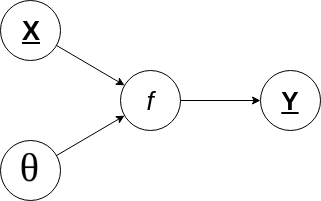
\includegraphics[width=50mm,scale=0.5]{images/FinalGraphicalModel.png}
  \end{center}
  
  Assumptions:
  \begin{itemize}
      \item We assume zero mean for the Gaussian prior and our assumptions about the nature of the function are encoded by our choice of kernel and the hyperparameters $\mathbf{\theta}$.
  \end{itemize}
  \begin{itemize}
      \item We have assumed that $\mathbf{Y}$ may not be completely determined by $\mathbf{X}$ and $f$, instead our likelihood function encodes the fact that $\mathbf{Y}$ may be corrupted by Gaussian noise.
  \end{itemize}
  \begin{itemize}
      \item We assume that $\mathbf{X}$ and $\mathbf{\Theta}$ are independent. How is this assumption justified? Based on our assumption that $\mathbf{X}$ and $\mathbf{\Theta}$ are independent we have that (7) can now be reduced to
      
    \begin{equation}
      p(\mathbf{Y},\mathbf{X},f,\mathbf{\Theta}) = p(\mathbf{Y}\mid\mathbf{X},f,\mathbf{\Theta})\cdot(p{f\mid\mathbf{X}, \mathbf{\Theta})}\cdot{p(\mathbf{X})}\cdot{p(\mathbf{\Theta})}
    \end{equation}
  \end{itemize}
  
  Annoyingly, we have added a new variable which we are not really interested in. Specifically we have modelled the relationship between $\mathbf{Y}$ and $f$ and also $f$ and $\mathbf{X}$ but what we are really interested in is the relationship between $\mathbf{Y}$ and $\mathbf{X}$. We should therefore marginalise out $f$ which involves computing the integral
  
  \begin{equation}
      p(\mathbf{Y}\mid \mathbf{X},\mathbf{\Theta}) = \int p(\mathbf{Y}\mid f)p(f\mid \mathbf{X},\mathbf{\Theta})df 
  \end{equation}
  
  \item{\large Question 11}
  Explain how this connects the prior p(f|x,O) and our data? (Ask Carl about that. What data does the question refer to?
  
  How does uncertainty 'filter' through the model?
  We have two causes of uncertainty in our model. The first cause of uncertainty is the choice of $f$, affecting our $f(x)$ term and the second second cause of uncertainty the additive Gaussian noise $\epsilon$ that is affecting our target variable $Y$.
  
  \begin{equation}
      \mathbf{y_i} = f(\mathbf{x_i}) + \epsilon
  \end{equation}
  
  Note that in (9), we have marginalised out $f$, however the uncertainty present in our choice of $f$ still remains. The uncertainty in $f$ is represented by the mean and the co-variance function defined by the kernel. This uncertainty 'filters' through when we marginalise out $f$. Our resultant distribution is then Gaussian, as both the likelihood and the prior are Gaussian. This concept of uncertainty 'filtering' through fits intuitively with the graphical model above, as after removing $f$, we still have that $Y$ is dependent on $X$ and $\theta$.
  
  The second cause of uncertainty, the additive Gaussian noise in our target variable $Y$, remains unaffected by the marginalisation of $f$. As can be seen in the equation (10), $\epsilon$ is completely independent of $f$, $\mathbf{X}$ and $\mathbf{\Theta}$.
  
  What does it imply that 0 is on the left hand side of the expression after marginalisation? After marginalisation, the LHS of (8) is given by $p(\mathbf{Y}\mid \mathbf{X},\mathbf{\Theta})$. From this expression we can see that Y is directly dependent on $\mathbf{\Theta}$ now that we have marginalised out $f$. Furthermore, the fact that $\mathbf{\Theta}$ is on the LHS of the expression implies that the values of the hyperparameters $\mathbf{\Theta}$ are already given and therefore we need not consider the distribution $p(\mathbf{\Theta})$.
  
  \item{\large Question 12}
  
  \begin{enumerate}
      
      We can assume that the prior $P(\mathbf{W})$ is a zero-mean isotropic Gaussian, hence $P(\mathbf{W})\sim N(\mathbf{W}|\mathbf{0},\alpha^{-1}\mathbf{I})$. Alpha can be...
      
      Picking alpha to be 2 we can visualise the prior as seen below:
      
    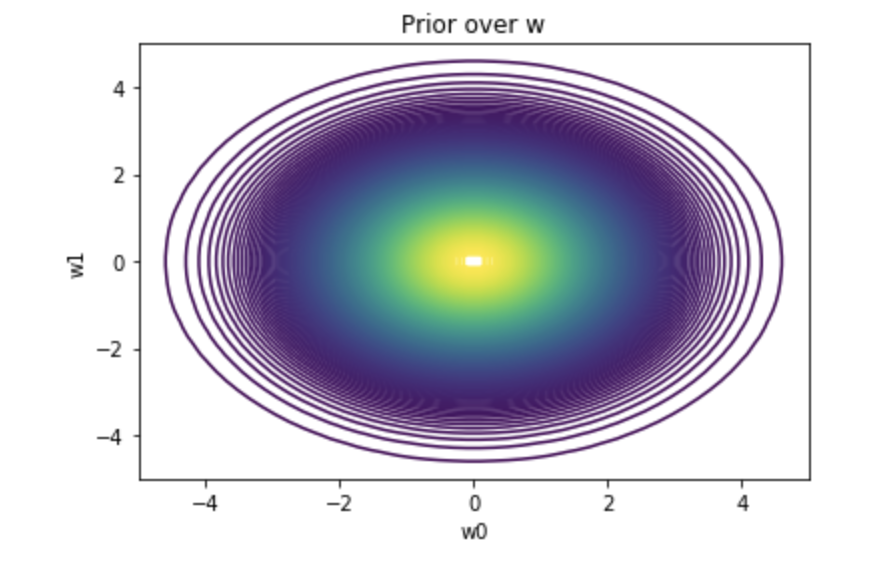
\includegraphics[width=50mm,scale=0.5]{images/priorw.png}
      
      The centroid is centred at (0,0) due to the mean being the zero vector. The horizontal and vertical principle axes are due to the spherical co-variance matrix specified in the prior. 
     
      Training our model with a single data point (-1, 2.0463131), we see that the model is generally imprecise with the sampled functions disagreeing wildly. We also see that the posterior distribution has large co-variance.
      
      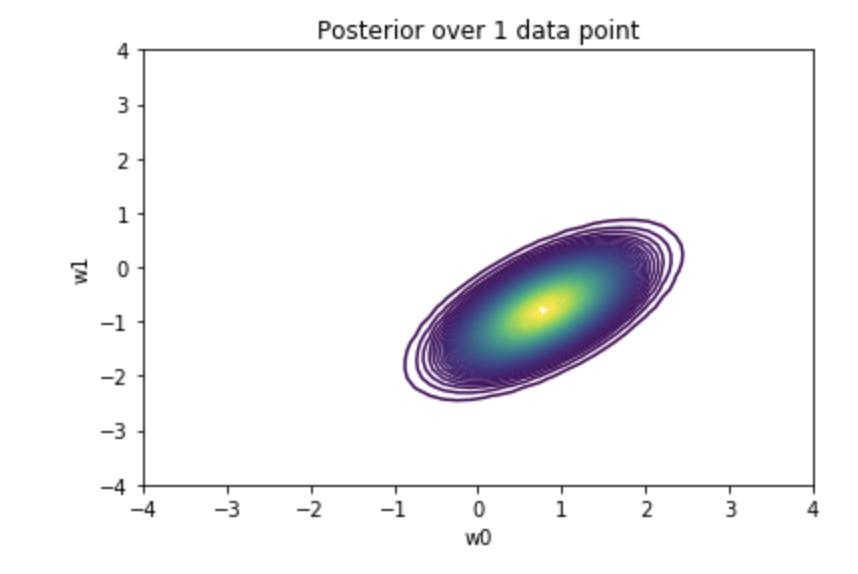
\includegraphics[width=50mm,scale=0.5]{images/post1.png}
      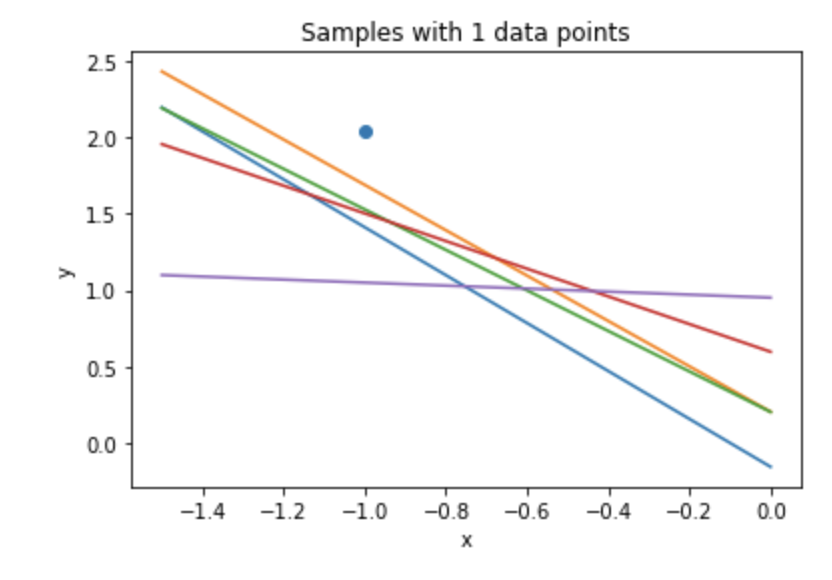
\includegraphics[width=50mm,scale=0.5]{images/sample1.png}
      
      Once 50 randomly selected data points are added, sampled functions begin to closely resemble one another and seem to fit the data points well.
      
      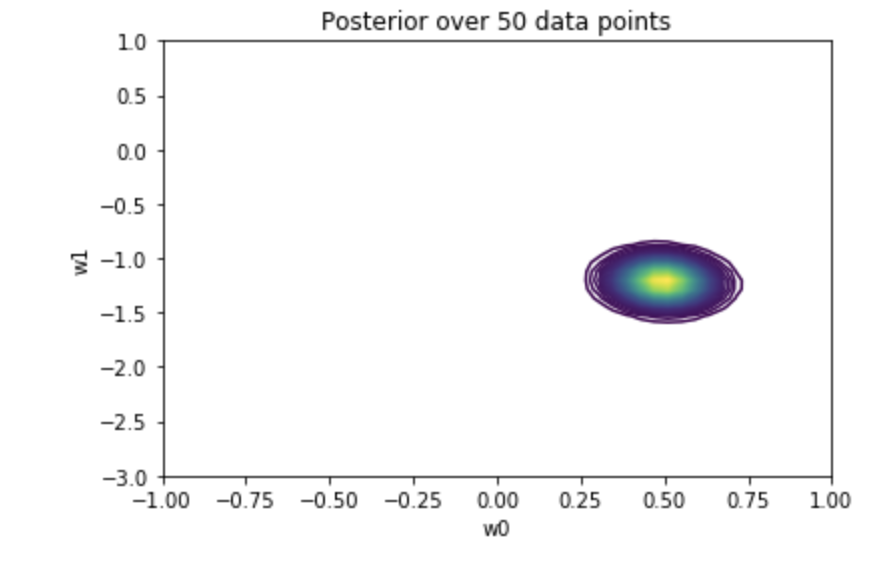
\includegraphics[width=50mm,scale=0.5]{images/post50.png}
      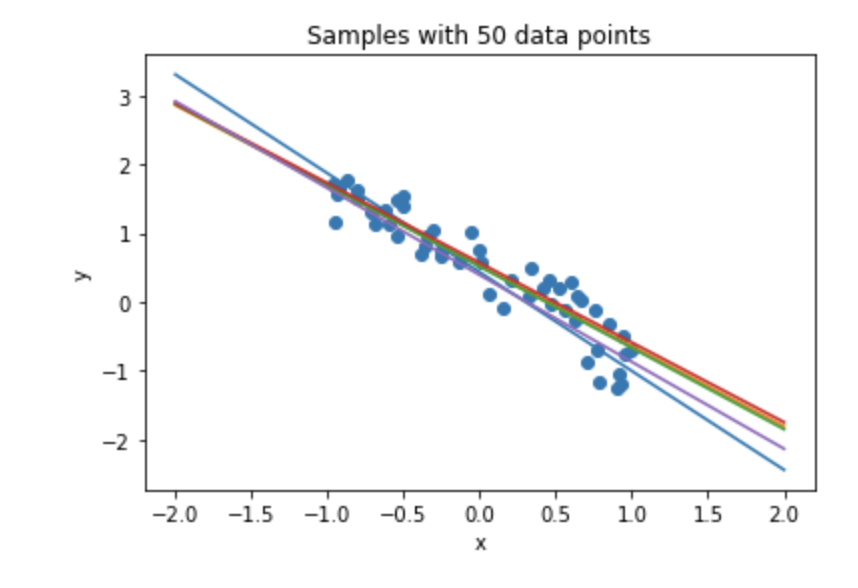
\includegraphics[width=50mm,scale=0.5]{images/sample50.png}
      
      It is  clear to see that the accuracy of the model is improved dramatically when it is trained with more data points. The co-variance between the weights has decreased.
      (what do you mean by this?)
      
      Relate to the expression of the posterior why you see the behaviour that you do when you add more data.
      Answer:
      
  \end{enumerate}
  
  \item{\large Question 13}
  Here we will implement and evaluate the effect of a Gaussian process prior with co-variance function
  
  \begin{equation}
      k(\mathbf{x_i},\mathbf{x_j}) = \sigma^{2}fe^\frac{-(\mathbf{x_i}-\mathbf{x_j})^T(\mathbf{x_i}-\mathbf{x_j})}{l^{2}}
  \end{equation}
  
  Where the $l$ is a hyper-parameter of the Gaussian process called the length-scale.
  
  2. Sample from this prior and visualise the samples with different length-scale for the squared exponential.
  
  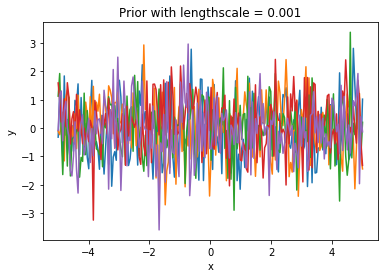
\includegraphics[width=70mm,scale=0.5]{images/GPPrior1.png}
  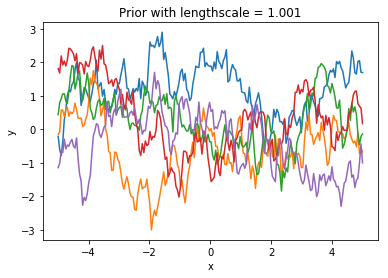
\includegraphics[width=70mm,scale=0.5]{images/GPPrior2.png}
  
  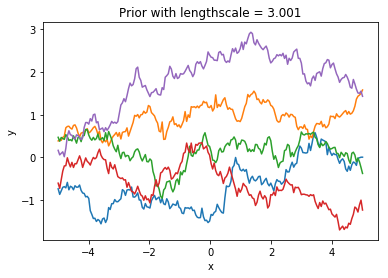
\includegraphics[width=70mm,scale=0.5]{images/GPPrior4.png}
  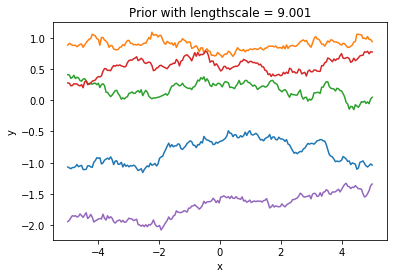
\includegraphics[width=70mm,scale=0.5]{images/GPPrior5.png}
  
  3.Explain the behaviour of altering the length-scale function. 
  We can see from (12) that as the value of the length-scale increases, the value of $k(\mathbf{x_i},\mathbf{x_j})$ also increases, meaning that $f(x_i)$ and $f(x_j)$ now co-vary more together. By increasing the length-scale, we ensure that values that are close together in input space will produce output values that are close together, giving a smoother function.
  
  4. What assumption does the length-scale encode?
   The length-scale encodes our assumption about the smoothness of the function.
  
  \item{\large Question 14}
  Using the prior from question 13 and introducing some data 
  
 1.Compute the predictive posterior distribution of the model
 
 2.Sample from this posterior with points both close to the data and far away from the observed data.
 
 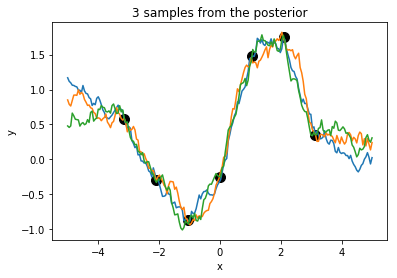
\includegraphics[width=70mm, scale=0.5]{images/GPPosteriorNoFudge.png}
 
 3.Plot the data, the predictive mean and the predictive variance of the posterior from the data.
 
 Explain the behaviour of the samples and compare the sample of the posterior with the ones from the prior. Is this behaviour desirable? what would happen if you added a diagonal co-variance matrix to the squared exponential?
 
 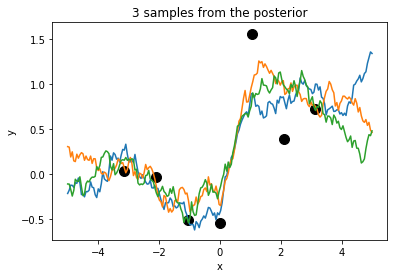
\includegraphics[width=70mm, scale=0.5]{images/GPPosterior.png}
  
  \item{\large Question 15: Elaborate on the relationship between assumptions, belief and preference.}
  
  Belief: "An acceptance that something exists or is true, especially one without proof."[oxford]\newline
  Assumption: "A thing that is accepted as true or as certain to happen, without proof."[oxford]
  
  Based purely on the definitions, beliefs and assumptions are equivalent and interchangeable. If the two concepts are truly equivalent, then there is little to say about how they relate to each other. We need not accept this equivalence, however. Perhaps beliefs and assumptions are distinct and we can view them as mutually dependent rather than equivalent? When we believe, we hold a certain proposition to be true (as given by the definition above). In doing so, one makes the \textit{a priori} assumption in the veracity of that belief and so beliefs require this \textit {a priori} assumption to even get off the ground.
  
  However, it is important to note that the assumption the belief relies upon is provisional. This means that there are two outcomes:
  \begin{itemize}
      \item The assumption will be ratified at some point in the future, when there is convincing evidence to confirm or refute the assumption, making it true or false.
  \end{itemize} 
  \begin{itemize}
      \item 2. The assumption will not be ratified.
  \end{itemize}
  If the assumption is ratified, then we can conclude whether or not our belief is true, as the foundation on which it is built will be shown to be stable or unstable. If, on the other hand, the assumption is not ratified, then no conclusions can be made as to the veracity of the belief.
  We must therefore accept that all beliefs are provisional because they are buttressed by provisional assumptions.
  
  How do preferences relate to both assumptions and beliefs? The idea of preference implies an ordering of some sort. Before any set can be ordered, each element must have some well-defined property which can be compared. Therefore, before a preference is specified, there must exist some beliefs about each of the elements. In this regard, preference can be viewed as the process of imposing a hierarchy on a set of beliefs.
  
  Now that the relationship between the three has been abstracted, it can be rooted in our machine learning example.
  
  When we perform machine learning algorithms, we already have beliefs about the world. We encode these beliefs in our assumptions about models that describe the world. More specifically, we have used prior distributions as a means of encoding our beliefs about a variable before seeing any data. (For preference speak about the choice of marginalising out X or W from our model and how in doing so we are valuing one variable over another, ie. Showing preference. In doing so we place a hierachical structure on our set of beliefs)
  
  \item{\large Question 16: What is the assumption/preference we have encoded with this prior?}
  
  A prior, $P(x) = N(0,I)$, encodes the assumption that all the dimensions are independent but encodes zero prior belief.

  \item{\large Question 17}
  page 93,156
  
  
  
  $$P(\mathbf{Y}, \mathbf{X}, \mathbf{W}) = P(\mathbf{Y}|\mathbf{X}, \mathbf{W})P(\mathbf{X})P(\mathbf{W})$$
  
  
  We marginalise out X
  
  $$P(\mathbf{Y},\mathbf{W}) = \int_{}^{} P(\mathbf{Y}, \mathbf{X}, \mathbf{W})  d\mathbf{X}$$
  
  
  $$P(\mathbf{Y},\mathbf{W})=  \int_{}^{} P(\mathbf{Y}|\mathbf{X}, \mathbf{W})P(\mathbf{X})P(\mathbf{W}) d\mathbf{X}$$
  
  $$P(\mathbf{Y},\mathbf{W})= P(\mathbf{W}) \int_{}^{} P(\mathbf{Y}|\mathbf{X}, \mathbf{W})P(\mathbf{X}) d\mathbf{X}$$
  
  $$P(\mathbf{Y},\mathbf{W})= P(\mathbf{W}) P(\mathbf{Y}|\mathbf{W})$$

  
  \item{\large Question 18}
  
  \begin{enumerate}
  
  
      \item{\Large  How are ML and MAP different?}
      
      Maximum a posteriori estimation takes into account prior beliefs as well as likelihood and tries to maximise the posterior whereas Maximum Likelihood is only concerned with the likelihood function
      
      Maximum likelihood estimation finds parameters that tries to maximise the likelihood function. It is essentially a special case of MAP estimation with the prior probability being uniform.
      
      Type 2 Maximum Likelihood estimations tries to find parameters that maximise the marginal likelihood.
      
      
      \item{\Large How are MAP and ML different when we observe more data?}
      
      
      
      When we have a substantial amount of data MAP and ML with converge to the same value(s)
      
      \item{\Large Why are the two expressions in Eq. 10 equal?}
      
      The denominator, $\int_{}^{} P(\mathbf{Y}| \mathbf{X}, \mathbf{W})P(\mathbf{W})  d\mathbf{X}$, is the marginalisation on W so is always positive and does not depend on W, hence plays no role in the maximisation problem.
  \end{enumerate}
  
  \item{\large Question 19}
  
  We can assume that the prior is of zero mean, that is:
  
  $$P(\mathbf{W}) \sim N(0, \mathbf{C})$$
  
  where $\mathbf{C}$ is some function on W producing the covariance matrix.
  
  Following this we can derive a log-likelihood function as follows:
  
  $$L(\mathbf{W}) = c + ln |\mathbf{C}| +  \sum_{i=1}^{\N} y_i^T\mathbf{C}^{-1}y_i $$
  
  We can then rewrite this and calculate the derivatives:
  
  $$L(\mathbf{W}) = c + ln |\mathbf{C}| +  tr(\mathbf{Y}\mathbf{C}^{-1}\mathbf{Y}^T)$$
  
  $$\frac{\partial L(\mathbf{W})}{\partial W_{ij}} = tr(\mathbf{C^{-1}}\frac{\partial \mathbf{C}}{\partial W_{ij}}) + tr(\mathbf{Y}\mathbf{Y}^T(-\mathbf{C^{-1}} \frac{ \partial \mathbf{C}}{\partial W_{ij}} \mathbf{C^{-1}})$$
  
  
  $$\frac{\partial L(\mathbf{W})}{\partial W_{ij}} = tr(\mathbf{C^{-1}}\frac{\partial \mathbf{W}\mathbf{W}^T}{\partial W_{ij}}) + tr(\mathbf{Y}\mathbf{Y}^T(-\mathbf{C^{-1}} \frac{ \partial \mathbf{\mathbf{W}\mathbf{W}^T}}{\partial W_{ij}} \mathbf{C^{-1}})$$
  
  
  
  \item{\large Question 20}
  
  Marginalizing over all unobserved variables requires an exponential number of computations.
  
  Suppose we have a directed chain of n variables with each variable able to take on z different values as seen below:
  
  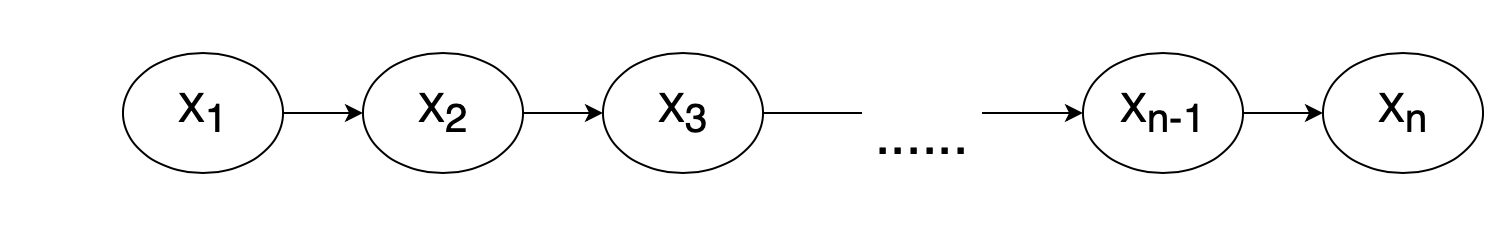
\includegraphics[width=100mm,scale=0.5]{images/q20.png}
  
  
  If we want to calculate \begin{equation} P(X_{n} = x) = \sum_{X_{1}...X_{n}}^{} P(X_{1}X_{2}...X_{n-1}X_{n}) \nonumber \end{equation}
  
  we have to marginalise over all variables $\{{X_{1}...X_{n-1}\}$ requiring $O(z^n)$ computations. When we have large sets of variables, this calculation quickly becomes computationally expensive.
  
   We can therefore define a general function $f$ such that
   $$f: \left(\{{X_{1}...X_{n-1}\} , \theta \right) \xrightarrow{} Y $$.
   
   Y now depends on $f$ and $f$ depends on $\{X_{n}\}$ and $\theta$. This means we can just marginalise over f whilst still utilising the information provided by {X{n}} and theta.
  
  Y depends on f, f depends on x and theta. If we marginalise out f then y is dependent on x and theta. (We explored this earlier in the CW)
  
  \includegraphics[]{}
  
  If we however marginalise out X then Y is dependent only on f and theta.
  Show this marginalisation and then show the model without X.
  
  We can see that as X has been marginalised out, Y is dependent on f which is in turn dependent on theta. WE have lost all uncertainty in X from our model and thus marginalising out X is analytically intractable.\\\\\\
  
 
  
  
  \item{\large Question 21 Plot the representation that you have learned. Explain why it looks the way it does. Was this the result that you expected? Hint: Plot X as a two-dimensional representation.}
  
  
  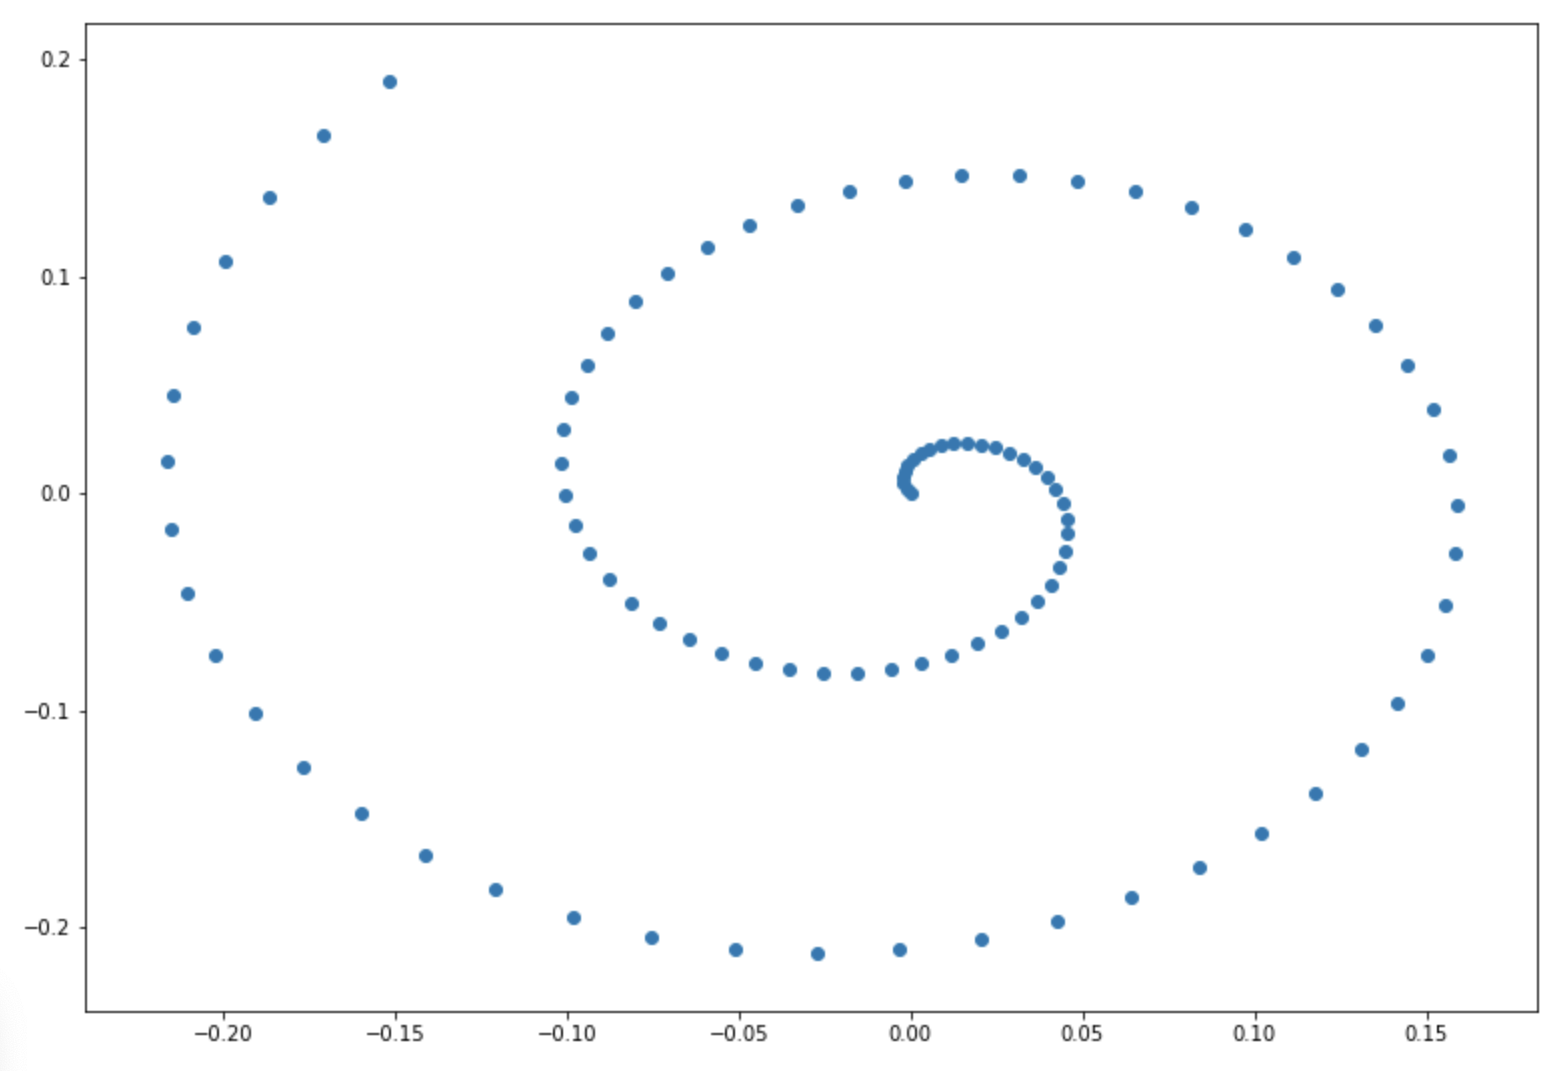
\includegraphics[width=50mm,scale=0.5]{images/q21.png}
  
  The points are in a spiral due to the parametric nature of the non-linear function. The function $ f_{non-lin}(x_{i}) = [x_{i}sin(x_{i}), x_{i}cos(x_{i})] $ essentially ...
  
  We did expect this result as if we were to plot $x sin(x),x cos(x)$
  
  
  \item{\large Question 22}
  
  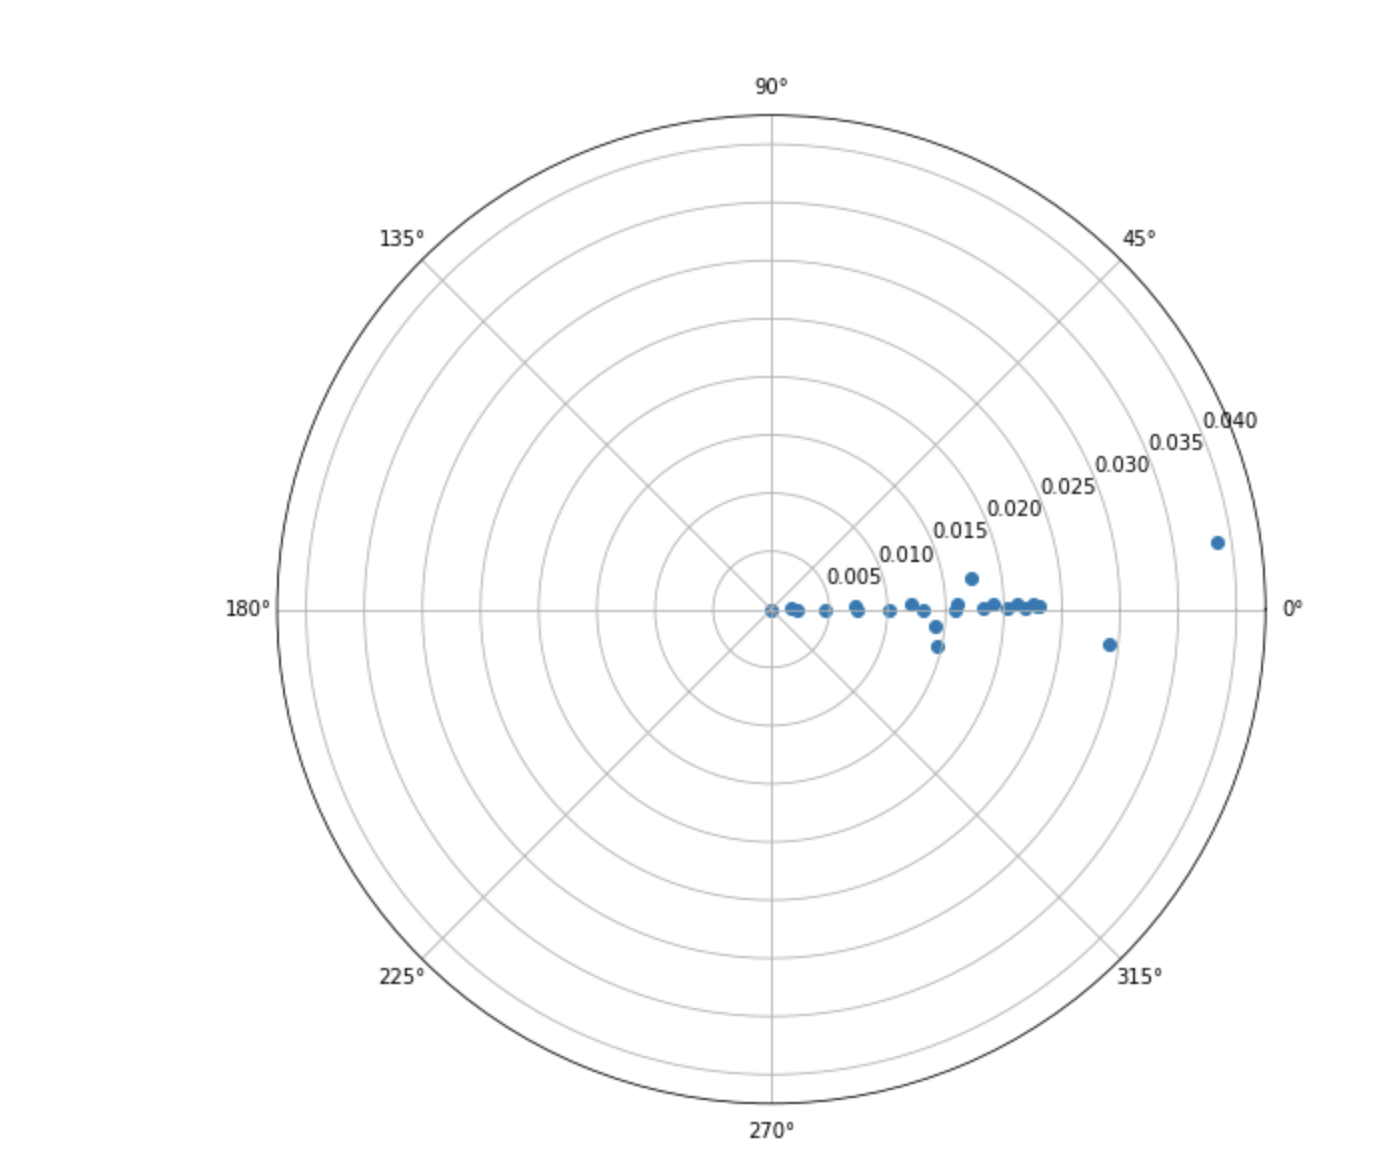
\includegraphics[width=50mm,scale=0.5]{images/q22polar.png}
  
  
  \item{Question 23}
  Why is it the most complex model? It has no flexibility about D. Doesn't depend on the value of $m_0$ or $\Theta_0$ and hence can't learn.
  Why is it the simplest model?
  
\end{enumerate}

TODO:
Draw a graphical models for Question 20
REDO The graphical models in the form that Carl does them

Question 1: finished (maybe Ask Kheeran about key factor argument)
question 2: finished
question 3: rewrite function with tilda and not = sign.
Question 4: write about the posterior and integrating to one (ask drew)
question 5: finished
Question 6: Need to copy out the derivation from adam's page.
Question 7: Some tidying to do
question 8: finished
question 9: finished
Question 10: Redo graphical model in Carl's form
Question 11: Part One
Question 12: Tidy                                                   
question 13: tidy                                                       DONE
question 14: Finish with Jake
question 15: Effectively finished, maybe tidy.
question 16: unfinished
question 17:
question 18: tidy
question 20: Draw graphical models in their proper form.
question 21: ask drew
question 22: ask drew



\end{document}
